\documentclass{article}

\usepackage[margin=1in]{geometry}
% \usepackage[noprefix]{nomencl}
% \usepackage[section]{placeins}
\usepackage[colorlinks,bookmarks,bookmarksnumbered,citecolor=red,urlcolor=red]{hyperref}
\usepackage{graphicx}
% \usepackage{cite}
\usepackage[caption=false]{subfig}

\begin{document}

\author{S. Andrew Ning}
\title{VAWT Aerodynamic Modeling}
\maketitle

\section{Introduction}
The aerodynamic analysis of vertical axis wind turbines (VAWTs) can be accomplished with simple methods based on blade-element momentum theory, more complex vortex methods, or detailed computational fluid dynamics (CFD).  The are an abundance of good CFD tools, and Sandia National Laboratories has developed a soon to be publicly available free wake vortex method (CACTUS).  These tools fill important roles in the design process, but simpler methods based on blade-element theory are useful for the conceptual design phase where a large range of designs need to be evaluated in a timely manner.

The application of blade-element theory to VAWTs results in a number of theories of increasing complexity: a single streamtube model, a multiple streamtube model, and a double multiple streamtube model.  The later approach is pursued in this project and is a good balance between computational speed and model fidelity for initial aerodynamic studies.

\section{Double Multiple Streamtube Method}
Double multiple streamtube theory allows for the VAWT blade path to be discretized in a 2-dimensional mesh, with separate momentum losses for both the upstream and downstream passes of the blade.  The method allows for complex blade geometry (curvature, sweep, pitch), wind shear, high-induction factors (Glauert correction), and any number of blades.

\begin{figure}[htbp]
\begin{center}
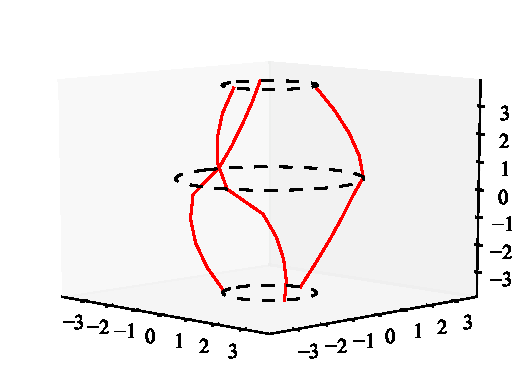
\includegraphics[width=3.5in]{geometry}
\caption{Isometric view of sample VAWT geometry.  All units in meters.}
\label{fig:geometry}
\end{center}
\end{figure}

As an example, a fictitious 3-bladed VAWT with a 5 meter diameter and 7.5 meter height is shown in Figure \ref{fig:geometry}.  The blades are constant chord with a solidity of 0.15 and NACA 0012 sections.  The normal and tangential loads for one blade are shown in Figure \ref{fig:loads}, and the variation in power coefficient with tip speed ratio in Figure \ref{fig:cp}.





\begin{figure}[htbp]
\centering
 \subfloat[Normal and tangential loads for one blade as a function of azimuthal position at a tip speed ratio of 5.0.  The upstream portion of rotation occurs from $\theta \in (-90, 90)$.]{
   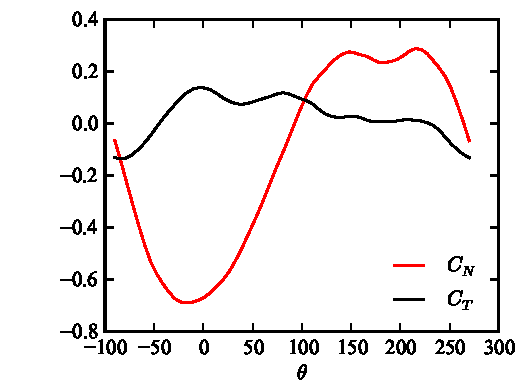
\includegraphics[width=0.45\textwidth]{loads}
   \label{fig:loads}
 }
 \qquad
 \subfloat[Power coefficient of entire turbine as a function of tip speed ratio.]{
   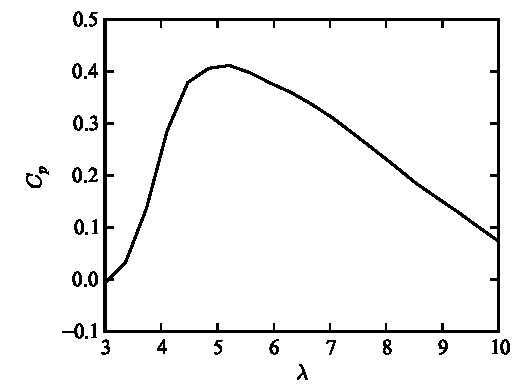
\includegraphics[width=0.45\textwidth]{cp}
   \label{fig:cp}
 }
 \caption{Loads and power coefficient of fictitious VAWT.}
\end{figure}


\end{document}